\subsection{Fizikus MI}
\begin{frame}{Fizikus MI}
    Eredeti cikk: \href{https://arxiv.org/pdf/1810.10525.pdf}{Toward an AI Physicist for Unsupervised Learning} \\
    Miért jobb az ember?
    \begin{itemize}
        \item Az adatok más forrásból jönnek $\rightarrow$ általánosítási problémák
        \item Nagy modellek bonyolultak
    \end{itemize}
    Megoldás: Egyesével megtanulni az egyszerű modelleket és rendszerezni \\
    Módszerek:
    \begin{itemize}
        \item Oszd meg és uralkodj: modell illesztése az adat egy részére
        \item Occam borotvája: legjobban illeszkedő modell kiválasztása
        \item Egyesítés: megtanult modellekből egy "mester elmélet" tanulása
        \item Élethosszig tartó tanulás: a tanult modelleket megjegyzi, később alkalmazza
    \end{itemize}
\end{frame}

\begin{frame}{Fizikus MI}
    \begin{columns}
        \begin{column}{0.45\textwidth}
            \centering
            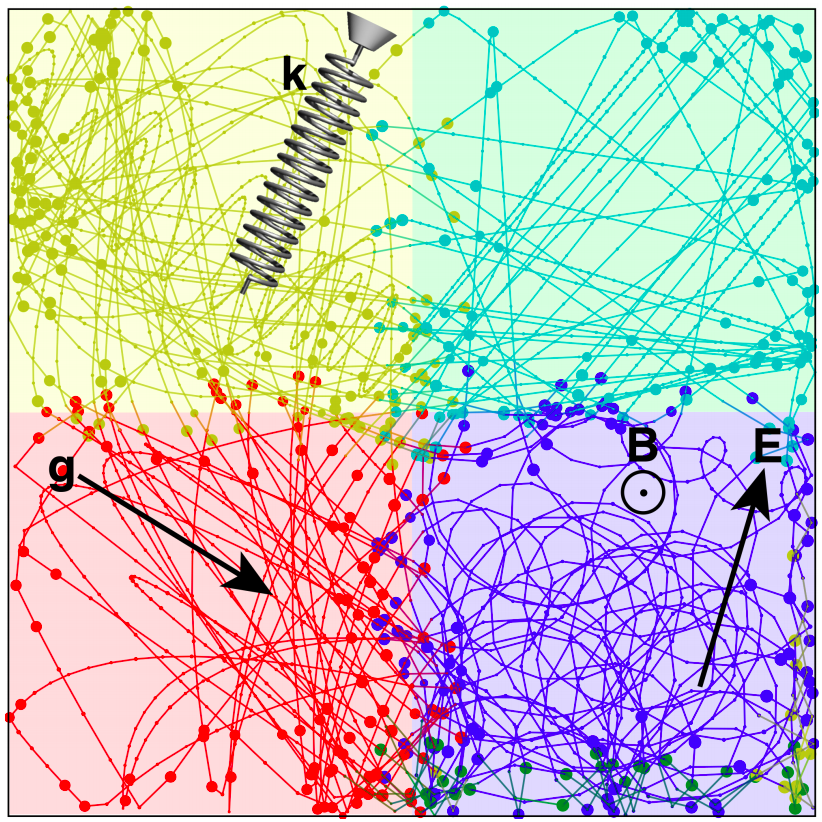
\includegraphics[width=1.0\textwidth]{figures/ai_phys_mystery_world.png}
        \end{column}
        \begin{column}{0.45\textwidth}
            Négy rész
            \begin{itemize}
                \item Harmonikus potenciál (sárga)
                \item Gravitációs mező (piros)
                \item Elektromágneses mező (lila)
                \item Rugalmas ütközés (cián)
            \end{itemize}
            Input: labda helyzete \\
            Cél: határok azonosítása és a mozgás leírása \\
            Pontok mérete: az előrejelzés hibája
        \end{column}
    \end{columns}
\end{frame}

\begin{frame}{Fizikus MI}
    Nehézség: 
    \begin{itemize}
        \item Könnyű problémákat tud megoldani
        \item Felügyelt tanulással osztályozási problémává válik a feladat $\rightarrow$ előrejelzés egyszerűen megoldható
        \item Valóság nem osztályozott: határokat a mozgással együtt kell megtanulni
        \item Előrejelzési hiba {\it nagyon} lecsökkent
        \item Kaotikus rendszerekre is működik ugyanilyen hibával
    \end{itemize}
    
    Általánosíthatóság:
    \begin{itemize}
        \item A négy paradigma a lényeg, nem a konkrét implementáció
        \item Analógia: Turing-gép (univerzális száámítógép, játékproblémákat old meg hatékonyan)
    \end{itemize}
\end{frame}